\chapter{Writing}
\label{ch:write}

\section{HTML}
\label{sec:html}

Have you ever seen a web URL like 
\begin{center}
\href{https://www.agnesscott.edu/lriddle/women/love.htm}{\tt https://www.agnesscott.edu/lriddle/women/love.htm}
\end{center}

\noindent and wondered what the \texttt{https} or the \texttt{htm}
meant? In both \texttt{https} and \texttt{htm}, the \texttt{ht} is
short for hypertext. The \texttt{tp} in \texttt{https} is short for
transfer protocol and the \texttt{s} is for secure. The \texttt{m}
in \texttt{htm} is for markup. All webpages, when it comes down to
it, are made of HTML (hypertext markup language) code. The HTML tells
the browser what should be displayed and, in general terms, the desired
layout. The browser takes care of the fine details depending on the
type of device, size of the screen, or personal preferences set by
the user.

Markup in HTML is like a note to the browser telling the browser how
to display the following content. The markup won't be displayed, but
it will modify how the content will be displayed. Take this screenshot
from \texttt{\href{https://www.southernct.edu/}{https://www.southernct.edu/}}
for instance.
\begin{center}

\includegraphics[width=4in]{SCSUscreenshot}
\par\end{center}

\noindent Simplified just a bit, the HTML code that produces the ``Back
to Campus'' announcement above looks like this:
\begin{verbatim}
<img src="/sites/default/files/back-to-campus-banner.jpg" /><p style
="font-size: 18px;">As the university prepares for the start of the
fall 2021 semester, we remain #SouthernStrong, with <a href="https://
inside.southernct.edu/reopening#services">all of the following academic
offerings and campus services</a> in place for our students in a safe,
engaging campus environment. Our goal is to get you off to a great
start, whether you're returning to campus or joining our community for
the first time!</p>
\end{verbatim}

\noindent It is just simple text! No bells, no whistles. Parts enclosed by \texttt{<}
and \texttt{>} are the markup. These parts will not be displayed themselves
but rather describe how something is to be displayed and leaves the
rest up to the browser. For example,

\begin{center}
\verb+<img src="/sites/default/files/back-to-campus-banner.jpg"/>}+
\par\end{center}

\noindent tells the browswer to insert an image ({\tt img}) and
tells the browser where to get the image ({\tt src}). This part
of the code creates

\begin{center}

\includegraphics[width=4in]{back-to-campus-banner}
\par\end{center}
  
\noindent The rest of the code creates the paragraph underneath this
image. It starts with \verb+<p style="font-size: 18px;" >+ --- which
tells the browser to start a paragraph ({\tt p}) using an 18 pixel
font---and ends with \verb+</p>+, which tells the browser this
is the end of the paragraph. In the middle of the paragraph is what
makes webpages webpages---a hyperlink. The text between 
\verb+<a href="https://inside.southernct.edu/reopening\#services" >+
and \verb+</a>+ is marked up as a link, it's displayed in blue so the reader can see that
these words are where they can click. Clicking them will bring up a new webpage in
the browser.
\clearpage

\begin{worksheet}{1}{Working with markup}{html.pdf}
To see markup in action, point your browser to 

\centerline{ \texttt{\href{https://htmledit.squarefree.com/}{https://htmledit.squarefree.com/}}, }

\noindent where you can write some hypertext markup and see how it looks on
your browser. The blue box at the top holds the markup, and it can
be edited by you! The box below shows how the browser renders the
markup. Do the following exercises on the \texttt{squarefree} webpage
and answer the questions.
\begin{enumerate}
\item Insert \texttt{<em>} before the word magically and insert \texttt{</em>}
after the word magically. What did this accomplish? Note: \texttt{em}
is short for \textit{em}phasis!
\item Copy and paste the following code into the webpage.

\begin{verbatim}
<p>A list of some common HTML markup
<ol>
 <li><tt>p</tt> is short for <b>p</b>aragraph</li>
 <li><tt>a</tt> is short for <b>a</b>nchor (which can
indicate a link or a place to link to)</li>
 <li><tt>ol</tt> is short for <b>o</b>rdered <b>l</b>ist</li>
 <li><tt>li</tt> is short for <b>l</b>ist <b>i</b>tem</li>
</ol>

Notice that markup can be nested -- the b and /b tags above are
inside the li and /li tags, which are between the ol and /ol
tags.</p>
\end{verbatim}


\item What happens to text between the \texttt{<b>} and \texttt{</b>} tags?
\item What happens to text between the \texttt{<tt>} and \texttt{</tt>}
tags?


\item Now change the \texttt{<ol>} and \texttt{</ol>} tags to \texttt{<ul>}
and \texttt{</ul>} tags. What happens to the displayed page (in the
white box)? Note: \texttt{ul} is short for \textbf{u}nordered \textbf{l}ist.

Make a new ordered list and use it to store your answers to the lab questions \#1, \#2, etc.

\item Notice how the b and /b tags in the last sentence of the copy/pasted code above are missing the usual angle brackets.  What happens if you put them in?
\item This is a problem in all markup languages -- some characters have special meaning.  In HTML there are so-called {\em escape characters} to work around this issue.  Google the phrase ``html escape characters'' and see if you can re-write the last sentence so that things {\bf look like} a tag, but don't {\bf act like} a tag!
\item Look up how to use the \texttt{<a href="...">...</a>} and \texttt{<img src="..."></img>} tags to make a link to another website and embed an image in your page.
\item Try writing some text and put a single \texttt{<br>} tag somewhere. What happens? Why doesn't it need a ``closing'' tag?
\item Similarly, what does the \texttt{<hr>} tag do?
\item There are lots of different computer programs (``browsers'') that need to translate the html source code of the webpages you visit into the beautiful layouts you see on your screen. How many different browsers can you think of?
\item Who is in charge of deciding what those browsers need to recognize as official html code? (Hint: search the internet for ``W3C.'') Who is in charge of that organization, and where do its profits go?
\end{enumerate}
\end{worksheet}

\section{LaTeX}
\label{sec:latex}

Donald Knuth is an amazing Zen master of Computer Science and Mathematics.  He created a program called \TeX{} (pronounced like ``tech'') for typesetting -- especially typesetting with mathematical content.  Knuth wrote \TeX{} mainly as an example of a style of coding that he called ``literate programming.''  Essentially this means that the programmer creates the documentation for their work at the same time they write the actual code.  Whether it's because of it being written in the ``literate programming'' style or simply because of Knuth's amazingness, \TeX{} is renowned as one of the most bug-free systems in existance. 

\TeX{}, and a follow-on program known as \LaTeX{}, which builds on \TeX{} and extends it, have become the standard(s) for communicating mathematics.  We'll be talking only about \LaTeX{}  from here onward.  \LaTeX{} is much like HTML -- it is a sort of markup language that gets processed and turned into a document suitable for visual display.  The appearance of \LaTeX{} source code is very different from that of HTML source code, but in many ways they are incredibly similar!  There are two marked distinctions:  HTML is meant to describe how to lay out a page so that the content is clear, and do so on many different displays -- the web-browser is empowered to alter things to aid in that clarity. On the other hand, \LaTeX{} is much more focussed on layout -- the first thing one does in a \LaTeX{} document is to specify the page size.  The author of a \LaTeX{} document can closely control where things will end up on that page\footnote{There is a strong argument against doing so -- the author should really concentrate on content, and let the software control the individual pixels on the page.}.
The other big difference between these systems is how well they handle mathematical content.  \LaTeX{} is very, very good at rendering mathematics and mathish notation from other fields like Chemistry.  HTML stinks at that, which is completely weird since the original HTML standard was created by a physicist at CERN, and physicists tend to use a lot of math\textellipsis

In a nutshell, HTML (the markup language of webpages) is used to
control how a webpage appears. \LaTeX{} plays the same role for printed
documents like books, reports, letters, or labs (like this one!).
\LaTeX{}   is a markup language that excels at creating technical documents,
especially those that include mathematical formulas. You might want
to read \href{https://medium.com/swlh/the-students-guide-to-latex-markup-what-it-is-and-why-you-want-it-651e723ce0c8}{this blog}
all about why you want to learn \LaTeX{}.

Like HTML, \LaTeX{} uses tags to mark how text should look, to insert
graphics, to create lists, and so on. Markup in \LaTeX{}   begins with
a \textbackslash{} (a backslash) as in {\tt \textbackslash pi},
which would be used to render our friend, $\pi$. Every \LaTeX{}  
document begins with the {\tt \textbackslash documentclass} tag,
which specifies what type of document is to be created (book, article,
report, etc.).  This is similar to HTML documents, which all begin with the \verb+<html>+
tag and end with the \verb+</html>+ tag. After the documentclass tag a \LaTeX{}   document must include the
tags {\tt \textbackslash begin\{document\}} and {\tt \textbackslash end\{document\}}.\footnote{This is similar to HTML documents, in which the beginning of the content
is marked by {\tt <body>} and the end by {\tt </body>}.} As you can probably guess, these tags mark the beginning and end
of the content of the document. One of the simplest \LaTeX{} documents
possible is this one:

\begin{codeblock}
\begin{verbatim}
\documentclass{article}
\begin{document}

Hello World!

\end{document}
\end{verbatim}
\end{codeblock}

Just like HTML code, it isn't pretty! However, it tells the \LaTeX{}  
renderer what to do. This code will create an ``article'' with the
sentence ``Hello World!'' in it. 

Let's give it a try!

The next lab will lead you through the process of creating \LaTeX{} documents on a web-based service known as {\em Overleaf}.

\clearpage
\begin{worksheet}{2}{Getting started with \LaTeX}{latex.pdf}
\begin{enumerate}
	\item Go to \href{https://www.overleaf.com/register}{\tt https://www.overleaf.com/register}
	\item Register for a free account (probably best to use your university email.)  You'll have to create a password at this point - make a note of it.\footnote{Overleaf isn't exactly a ``high stakes'' setting, your password needn't be super complicated -- just don't re-use a password that protects a more critical account!}
	\item It's probably best to skip their ``Try the premium version for free'' offer.
    \item Click the ``Create First Project'' button -- choose a blank project and name it ``hello.''
    \item You'll see two main panels (there's also some junk above and to the left, but ignore all that for now.)  The left-hand panel contains the \LaTeX\ source code for your project and the right-hand panel gives a preview of the resulting document.
    \item The ``blank project'' isn't completely blank.  The source code panel will be pre-populated with:
\medskip

\begin{codeblock}
\begin{verbatim}
 \documentclass{article}
 \usepackage{graphicx} % Required for inserting images

 \title{hello}
 \author{myemail}
 \date{August 2023}

 \begin{document}

 \maketitle

 \section{Introduction}

 \end{document}
\end{verbatim}
\end{codeblock}

\clearpage

You should see your document on the right side. It has a title section (which is 
what the \verb+\maketitle+ command created) and a section heading (this is what the \verb+\section{Introduction}+ command did). Scroll down to the bottom of the page and you
will see the number 1, the page number. Pages of articles are normally
numbered, so \LaTeX\  puts that in for you!  The area
between the \verb+\documentclass{article}+ and
the \verb+\begin{document}+ tags is known
as the \textbf{preamble} of the \LaTeX\  document. 
You should see that the preamble contains some commands that effect how the title looks.  
The default stuff that Overleaf stuck in there probably isn't quite what you want.

Let's fix that!


\item Make whatever changes you deem appropriate to the title, author and date commands. (BTW, ``date'' doesn't necessarily have to literally be the date.)  To see what the effect of your changes is, you'll need to press the ``Recompile'' button.

\item Put some words, introducing yourself after the \verb+\section{Introduction}+ command, and recompile. (There is an old and slightly unfunny tradition that the first program you write when learning a new programming language is called ``hello world!''  Please make your introduction something other than that.)

\end{enumerate}

At this point the source code might look something like:
\bigskip

\begin{codeblock}
\begin{verbatim}
\documentclass{article}
\usepackage{graphicx} % Required for inserting images

\title{My first LaTeX document}
\author{Ima Dumi}
\date{just checking that I can put whatever I want in the date}

\begin{document}

\maketitle

\section{Introduction}

Something other than that.

\end{document}
\end{verbatim}
\end{codeblock}

\clearpage

Which should render like so:


\begin{center}
\fbox{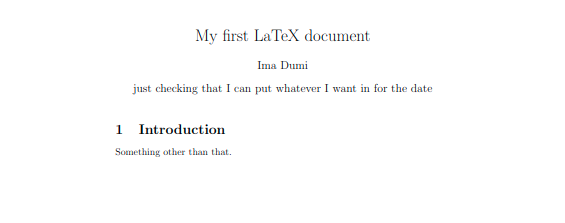
\includegraphics[width=6in]{HelloWorldScreenshot.png}}
\end{center}


\subsection*{Adding a list}

Now add a list of your three favorite classes of all time---of course
math class is first on your list, so that one has been put in for
you. You'll have to supply the next two...

\begin{enumerate}

\item Copy and paste the following markup into your document 
after your greeting, but before \verb+\end{document}+.
\bigskip

\begin{codeblock}
\begin{verbatim}
\par
My three favorite classes of all time are

\begin{enumerate}
  \item Math
\end{enumerate}
\end{verbatim}
\end{codeblock}
\bigskip

Notice that the \verb+\par+ tag does not have a begin
or end. It only marks where a new paragraph should start. Same with
the \verb+\item+ tag. It only marks where a new item
in the list should start.
\item Add two items to the enumeration (and you can change the first item
if by some strange chance math is not your all time favorite class).
\item There are several list-making environments in \LaTeX.  Try some googling (Maybe ``list making latex environments'') 
and you should discover the other list-making environments.
\item Make version of your list of favorite classes that are (1) bulleted rather than numbered, (2) name the class and also give a comment about \sout{why math is so awesome} why you like it.

\end{enumerate}

\subsection*{Adding an equation}

Equations in \LaTeX\ come in two varieties---inline and display.
An inline equation is any mathematical expression that appears in
the middle of a sentence (like the $\pi$ right here and earlier in
this document). A display equation is any mathematical expression
that should appear centered on its own line (because it's super important
or just because it's too big to put in the middle of a sentence).

To put an equation in the middle of a sentence, enclose the math between
two dollar signs (\$). To add a display equation, enclose the math
between double dollar signs (\$\$). Try it!

\begin{enumerate}
\item Copy and paste the following markup into your document.
\bigskip

\begin{codeblock}
\begin{verbatim}
My favorite mathematical constant is $\pi$, but I like $e$ too.
Did you know that $$e^{i\pi}=-1?$$ Weird...
\end{verbatim}
\end{codeblock}
\bigskip

\item Notice that exponents are typeset using the same notation as used
on a calculator! Can you add markup to your document that will produce
the following?

\begin{quote}
The Pythagorean Theorem states that if a triangle has legs of lengths
$a$ and $b$ and hypotenuse of length $c$, then
\[
a^{2}+b^{2}=c^{2}.
\]
\end{quote}

\end{enumerate}

\end{worksheet}

\section{More LaTeX}
\label{sec:more_latex}

Before we get to working a bit more with \LaTeX{}, let's do some configuring that will save you a little typing going forward.
When you create a new project in Overleaf, the system automatically puts your name in as the document's author.  Unfortunately, it usually doesn't get your name right.  Click the ``home'' icon (in the upper left, next to ``Menu'').  There is a drop-down labelled ``Account'' select ``Account Settings'' from it and then fix your first and last names.

Now if you create a new blank project, the preamble of your new documents should look something like this:

\begin{codeblock}
\begin{verbatim}
\documentclass{article}
\usepackage{graphicx} % Required for inserting images

\title{hello}
\author{Joe Fields}
\date{August 2023}

\end{verbatim}
\end{codeblock}

Notice that commands all start with a backslash followed by the command name, followed by something in curly braces.  Well, not quite -- the thing in curly braces (a.k.a french braces) is called the argument of the command -- some commands don't have arguments, others have more than one. So the very first thing in the preamble is a {\tt documentclass} command, whose argument is the word ``article.''  Often such a command will also have optional arguements -- these are collected in square braces between the command name and the curly brace arguments.

For example:

\begin{codeblock}
\begin{verbatim}
\documentclass[12pt]{article}

\end{verbatim}
\end{codeblock}

Would make an article with a slightly larger font.  (Font styles and size can be set inside the document too.)  There are quite a few other optional arguments available.

The second line of the preamble has a couple of things worth mentioning.  The first is that there is a comment.  Any text after a \% sign is ignored, so this gives you a way to write little ``note-to-self''s.  The second is what the line is doing -- adding to the default behavior of latex.  There is a large community of \LaTeX{}   users who actively develop new features.  These features are made available through {\em packages}.  

The \LaTeX{}   source for this book makes use of a lot of packages: 
hyperref, geometry, fncychap, babel, makeidx, graphicx, rotating, amssymb, amsmath, amsthm, color, and ulem.  We'll explore a couple of those in the lab.


\clearpage
\begin{worksheet}{3}{More with \LaTeX}{latex.pdf}
\begin{enumerate}
	\item Did you fix your name in the Overleaf ``Account'' area?
	\item Okay. Then, start a new blank project called ``more''
	\item Edit the first line of your new project to include an optional argument for the \verb+\documentclass+ command:
	\medskip

\begin{codeblock}
\begin{verbatim}
	\documentclass[12pt]{article}
\end{verbatim}
\end{codeblock}
\medskip

	\item Also, add the following lines into the preamble of your document:
\medskip

\begin{codeblock}
\begin{verbatim}
%\usepackage{geometry}
%\usepackage{hyperref}
\end{verbatim}
\end{codeblock}

Of course, the commands you've just entered start with the comment symbol so they won't {\em do} anything.  Did you notice how the Overleaf source editor renders them in green?

	\item Now, add the following to the body of your document.  (After the \verb+\section{Introduction}+ command)
\medskip

\begin{codeblock}
\begin{verbatim}
The first thing you should notice is that the text is a little
bigger than it was last time.  You may also have noticed that 
the margins are a bit big by default.  For illustration purposes 
we need a paragraph that is long enough to ensure we've 
reached the right margin.  This one should do the trick.
\end{verbatim}
\end{codeblock}
\medskip

	\item Hit the ``Recompile'' button.  Did you notice that the text is a little bigger than it was last time?
	\item Try deleting the \verb+[12pt]+ optional argument to the \verb+\documentclass+ command.  Hit ``Recompile.'' Do you see the difference now?  
	\item Put the \verb+[12pt]+ optional argument back and recompile one last time.
	\item Okay, now what about that comment about \LaTeX{}'s margins?  Try uncommenting the line that includes the {\tt geometry} package.
	Recompile.  What's changed?
	\item The {\tt geometry} package will give you minute control over your document's margins.  The default margins when the {\tt geometry} package is in use are a good bit smaller than \LaTeX{}'s defaults.
	\item Try replacing the {\tt geometry} line with this one:
\medskip

\begin{codeblock}
\begin{verbatim}
\usepackage[bottom=1in, right=.5in, left=.5in, top=1in]{geometry}
\end{verbatim}
\end{codeblock}
\medskip

    \item Play around a bit.  What settings for the margins are most pleasing to your eyes?
    \item Now, uncomment the \verb+\usepackage{hyperref}+ command.  Recompile.
    \item Did you see anything change?
    \item If you did, it's probably your imagination. Hyperref doesn't make any visible changes -- it provide you with some new commands!
    \item Drop the following line into your source file:
\medskip

\begin{codeblock}
\begin{verbatim}
This is a 
\href{https://www.cespedes.org/blog/85/}{link} 
to a page that gives some good information about 
special characters in \LaTeX{}.  You may notice 
that the {\tt href} command provided by the 
{\tt hyperref} package is our first example of a 
\LaTeX{} command that has two arguments.
\end{verbatim}
\end{codeblock}
\medskip

	\item I don't know about you, but I really don't like how hyperlinks are rendered by default.  If you put the following right after the \verb+\usepackage{hyperref}+ command you'll get a nicer appearance.
\medskip

\begin{codeblock}
\begin{verbatim}
\hypersetup{colorlinks=true,  urlcolor=blue}
\end{verbatim}
\end{codeblock}
\medskip


\end{enumerate}

\end{worksheet}
\clearpage

\section{even more LaTeX}
\label{sec:even_more_latex}

There's a term you'll hear in the publishing world and sometimes in Computer Science: whitespace.
It's a collective term for all of the symbols that don't end up putting ink on the page. Basically, the whitespace characters are: the space key, the tab key, and the Enter key.  In \LaTeX{}  the only thing whitespace characters do is seperate the printable things (ordinary characters and \LaTeX{}  commands).  In particular, they don't add extra space!  You can put a single blank line between two paragraph, or you can put 27 blank lines.  The output will look the same.  THIS CAN BE MADDENING!  You notice that an inline equation looks a little pinched in too close to the surrounding text, so you put in some extra spaces, and it has no effect.  So you put in some more spaces, and still nothing happens.  They say insanity consists of repeating the same experiment expecting different results.  Try not to travel too far down that path!  Maybe repeat the mantra ``whitespace is just whitespace'' while you're doing the next lab -- don't expect it to produce actual space\textellipsis

So, how {\em do} we produce actual space?  How do we fine tune the space between things?  (This might mean adding or {\em subtracting} space.)

First, you should probably ask yourself if the change you want is really desireable.  \LaTeX{}  has some pretty good algorithms for calculating spacing\textellipsis

Second, you should check if there's a systematic way to make the change you want.  For instance, if you want a little additional space between your paragraphs, you can put something in the preamble that adjusts those inter-paragraph spaces throughout the document:

\begin{codeblock}
\begin{verbatim}
\setlength{\parskip}{8pt}
\end{verbatim}
\end{codeblock}

\noindent or, if you want your whole document to be double-spaced:

\begin{codeblock}
\begin{verbatim}
\linespread{2.0}
\end{verbatim}
\end{codeblock}

But, if you really want fine-grained control there are commands for adding vertical and horizontal space:

\begin{codeblock}
\begin{verbatim}
Hickory dickory dock \hspace{1in} The mouse went up the clock.

      % There should be blank lines surrounding the space command              
      % Cutting and pasting might leave them out, so add them
      % back in if they're missing.

\vspace{.5in}
                
The clock struck one. The mouse went down. Hickory dickory dock
\end{verbatim}
\end{codeblock}

Will give output that looks like this:

\begin{center}
\fbox{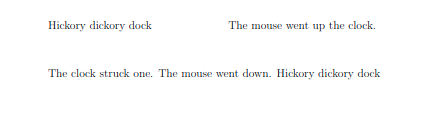
\includegraphics[width=6in]{Hickory.png}}
\end{center}

In math mode there are special spacing commands (\verb+ \,  \;  \!  \quad+) that we can use to make finicky adjustments to the positions of symbols.  

If all else fails there are struts.  \LaTeX{} has a command that's meant to create a rectangular blob of ink -- 
\verb+\rule{width}{height}+, but if you make one of those lengths $0$ the resulting blob won't have any ink in it -- it'll be an invisible thing that just takes up space -- that's called a strut.  I sincerely hope you don't find yourself creating struts in this course.  They're really frowned upon -- there's almost always some better way of handling things than making an invisible space-taking-upping thing.  Just thought you should know, 'cause sometimes\textellipsis

\clearpage
\begin{worksheet}{4}{More more with \LaTeX}{latex.pdf}
\begin{enumerate}
	\item Go to Overleaf and, instead of a blank project, under New Project select ``Example Project.''

  \item Take a little time to go through the source code line-by-line and figure out what things do.

  \item Try the following matching exercise.

 \hspace{-.75in} \begin{tabular}{lcl} 
 & \rule{48pt}{0pt} & \\
\rule[-18pt]{0pt}{48pt} \begin{small}\verb+\href{https://www.overleaf.com/learn}{help library}+ \end{small} & & A. Set the author field \\
\rule[-18pt]{0pt}{48pt} \begin{small}\verb+\author{You}+ \end{small} & & B. A hyperlink\\
\rule[-18pt]{0pt}{48pt} \begin{small}\verb+\includegraphics[width=0.25\linewidth]{frog.jpg}+ \end{small} & & C. Start a numbered list\\
\rule[-18pt]{0pt}{48pt} \begin{small}\verb+\url{https://www.overleaf.com/contact}+  \end{small} & & D. Some displayed math\\
\rule[-18pt]{0pt}{48pt} \begin{small}\verb+\usepackage[english]{babel}+ \end{small} & & E. Puts in an image\\
\rule[-18pt]{0pt}{48pt} \begin{small}\verb-\begin{enumerate}- \end{small} & & F. Sets the document language\\
\rule[0pt]{0pt}{30pt}   \begin{small}\verb-\[S_n = \frac{X_1 + X_2 + \cdots + X_n}{n}- \end{small} & & G. An alternative form\\
\rule[-18pt]{0pt}{30pt} \begin{small}\verb+    = \frac{1}{n}\sum_{i}^{n} X_i\]+ \end{small} & & \hspace{.2in} of a hyperlink\\
\end{tabular}

\clearpage

\item You may have notice the use of \verb+\[+ and \verb+\]+ to begin and end the display math environment.  Using \verb+$$+ to begin and end a displayed math environment (or \verb+$+ to begin and end an inline math environment) has an unfortunate consequence.  Users have a tendency to forget either the begin or the end tag which leads to errors at compile time that are really hard to figure out.  If you get compilation errors that seem plain crazy, check to see if every `begin math' token has a matching `end math' token.  The problem is a little easier to deal with when the begin and end tags are different.

The begin/end version of the tags for displayed math are \verb+\[+ and \verb+\]+.

The begin/end version of the tags for inline math are \verb+\(+ and \verb+\)+.

So, either use these -- or take my advice and learn to scan your code for mismatched dollar signs!

\centerline{\rule{2in}{.5pt}}

Next we're going to explore more of the features of the Overleaf interface.  The panel to the left of the `Edit' panel contains two subparts, above is a file listing.  The current project has 3 files in it.  The sub-panel below shows the logical structure of the document - you can click on things to move to the spot in the source code where they are defined.  The panel that runs along the top of the page contains the Overleaf menu and the Home button on the left and towards the right we see Review, Share, Submit, History and Chat.  Let's start with Share.

\centerline{\rule{2in}{.5pt}}

\item Find a partner, one of you create a new project (use the Example Project template again) then share it with the other.  If you both go to the Home area in your respective instances of Overleaf, you should each be able to see the project.  You should be able to edit the project simultaneously!  

\vfill

\item One of you should adjust the \verb+\author{}+ command so that it contains both your names.  The other should add a comment to the file, maybe ``I think my name should be first.''  To add a comment, click the Review button which opens a new panel between the source and the pdf panels -- highlight some text in the edit panel and you'll be prompted for your comment.

\vfill 

\clearpage

\item The Overleaf interface contains elements for resizing and hiding the various panels.  Play around with customizing the interface.  (For instance I often work with only the Edit and Review panels open - then I just need to unhide the Pdf panel when it's time to recompile and see how my changes look.)

\vfill

\item When working collaboratively, but not physically near one another, the Chat panel can be quite useful.  Send each other a chat!

\vfill

\item One last thing.  Did you notice how the size of the little frog image was specified?  You can also use an actual length, but the strategy used here (making the image's width be a percentage of the width of a line) is smart.  Other possibilities are to give a scale factor:

\begin{codeblock}
\begin{verbatim}
\begin{figure}
\centering
\includegraphics[scale=.25]{frog.jpg}
\caption{\label{fig:frog}This frog was uploaded via the file-tree menu.}
\end{figure}
\end{verbatim}
\end{codeblock}

Make that change and recompile.

\vfill

\item You should notice that the frog picture is somewhat bigger, and also that it appears in a different place!  That's because things like tables and figures are known as ``floats.''  The typesetter (in this case the \LaTeX{} software) has considerable latitude about where they end up in the layout.  Because it's possible that a table or figure ends up far from where it's referred to in the text, these ``floats'' are usually numbered.  As you work and revise a document, it's quite possible for new diagrams and tables to move things about and change those numbers.  Look for the commands \verb+\ref{}+ and \verb+\label{}+ in the source code to see how \LaTeX{} can automatically keep these number references current (with a little help from the author).

\vfill

\clearpage

\item Notice that in one part of the current project there is an example of a simple table.  Create a new section, and add a table to your document which tabulates some data you get from 3 or 4 classmates:  name, favorite animal, favorite color, favorite automobile -- actually, pick your own favorite somethings!  Use the ``table'' environment as a container for your table (which should be created using the ``tabular'' environment)
make sure that the table has an appropriate caption and that there is a \verb+\label{}+ command.  The typesetter may decide to put your table somewhere else in the document!  Write a short paragraph about all this stuff and include a \verb+\ref{}+ to your table.

\end{enumerate}

\end{worksheet}
\clearpage

\section{MathJax}
\label{sec:mathjax}

\LaTeX{} is getting somewhat dated.  It seems likely that it'll be supplanted by something more user-friendly at some time during your professional career.  Still, the notation that \LaTeX{} uses to encode mathematical content works incredibly well.  It pops up in unexpected places.  For instance, when Mathematicians and/or Scientists are communicating via email, and some math needs to be expressed, out come the dollar signs!  The object of study in this section is MathJax -- a javascript package that allows one to include mathematical content into webpages.  Perhaps it won't be surprising to learn that \LaTeX{} math notation is involved!

Unfortunately, the sandbox where we played with HTML markup previously doesn't allow for scripting (and MathJax is a script) so we will need to work in a more permissive environment.  Google makes a free service called Sites available to the public.  This is ``free as in beer'' not ``free as in liberty'' but still, it's pretty cool that they make something available to the general public that lets folks create websites in a (more or less) ``What You See Is What You Get'' environment.  But, there is a bit of a backdoor!  One can also drop arbitrary HTML code into a Google sites page.  

That's where we are going in the next lab.

\clearpage
\begin{worksheet}{5}{MathJax}{MathJaxLogo.png}
\begin{enumerate}
	\item To do this lab, you'll need a free Google account.  If you don't have one and are unwilling to sign up for one, your instructor may be able to provide you with login credentials for a dummy account.
	\item Verify that you are signed in to your Google account (for instance check if you can see your ``Gmail'' email.)
	\item Point your browser to \url{sites.google.com} and start a new, blank, site. 
  \item On the right-hand side of the screen there is a menu system containing a variety of elements you can add to your site.  Select the one that says ``Embed.''  In the dialog that pops up, switch it over to ``embed code'' and paste the following into the text box:
\begin{codeblock}
\begin{verbatim}
<!DOCTYPE html>
<html>
<head>
    <meta charset="utf-8">
    <title>MathJax Example</title>
    <script id="MathJax-script" async
          src="https://cdn.jsdelivr.net/npm/mathjax@3/es5/tex-mml-chtml.js">
    </script>
</head>
<body>
<H2> Testing MathJax </h2>
<p>
If we are given a quadratic polynomial \(Ax^2+Bx+C\), we can find its zeros 
using the quadratic formula, a relatively simple expression in terms of the 
coefficients \(A\), \(B\) and \(C\) which gives the \(x\) values that satisfy 
\(Ax^2+Bx+C = 0\).
<p>
The formula is
\[ \frac{-B \pm \sqrt{B^2 - 4AC}}{2A}. \]
</body>
</html>
\end{verbatim}
\end{codeblock}

\item If you want to make changes to your embedded element, click somewhere in it (to select it) and notice the icons that appear in the upper-left corner.  Select the pencil to edit.  Also, the text area that contains your code is very tiny, but it has a resizing handle in the bottom right corner.

\item Turn your attention to the tool area at the top of the window towards the right.  The first three icons there are ``undo,'' ``redo,'' and ``preview.''  It's probably obvious that undo and redo are useful!  The preview button is pretty cool too, it let's you see how your site will appear on a regular computer, or on a tablet or cellphone.  The blue X leaves preview mode.

\item We've basically just hijacked Google sites to create a sandbox for playing around with \LaTeX{} math!  A lot of people prefer to use the \$\dots\$ notation for math.  You can enable that by adding the following magic spell to your preamble:
\begin{codeblock}
\begin{verbatim}
  <script>
    window.MathJax = {
        tex: {
            inlineMath: [['$', '$'], ['\\(', '\\)']]
        }
    };
  </script>
\end{verbatim}
\end{codeblock}
\item Try the following.  Count on your fingers but doubling with each step instead of adding 1 with each step. 
\begin{enumerate}
  \item 2
  \item 4
  \item 8
  \item 16
\end{enumerate}
{\it et cetera}

Of course, repeated multiplication is the same thing as exponentiation, so if you made it through all ten of your fingers, you should know the value of $2^{10}$.  You could also work backwards (cutting in half with each step) to figure out the value of $2^0$.  Or you could enlist a friend and work out what $2^{20}$ is.

Create a little webpage - using MathJax for the math - explaining all this for someone who's in, say, Middle School (maybe 6th or 7th grade).  See if you can use the intuition from this physical activity to explain that weird rule about powers: $a^b \cdot a^c = a^{b+c}$.
\end{enumerate}

\end{worksheet}
\clearpage


%\section{More Markup (Blogs and Wikis)}
%\label{sec:markup}

%% Move the Markup section into the CAS chapter.
